\documentclass[11pt,a4paper]{article}
\usepackage[utf8]{inputenc}\usepackage[T1]{fontenc}
\usepackage[margin=1in]{geometry}
\usepackage{amsmath,amssymb,booktabs,graphicx,enumitem,xcolor,parskip,titlesec,multirow}
\usepackage[hidelinks]{hyperref}
\graphicspath{{figures/}}
\definecolor{qnavy}{RGB}{20,40,75}\definecolor{qgrey}{RGB}{90,90,90}
\titleformat{\section}{\large\bfseries\color{qnavy}}{\thesection}{0.6em}{}

\begin{document}
\thispagestyle{empty}
\noindent
{\large\bfseries\color{qnavy} Report R02 --- Radiomics and Overall Survival in Glioblastoma}\\[2pt]
{\color{qgrey}A positive prognostic result, with the positive controls R01 lacked.}\\[6pt]
{\color{qgrey}\rule{\textwidth}{0.4pt}}

\medskip
\noindent 7 August 2026 \quad\textbullet\quad Quantara \quad\textbullet\quad
Companion to R01 (MGMT classification, null)

\section*{Summary}

Radiomic features from routine preoperative MRI \textbf{do} carry prognostic information
about overall survival in UPENN-GBM: Harrell C-index \textbf{0.602} (95\% CI 0.576--0.629),
permutation $p = 0.005$, on 574 patients. The signal is \emph{independent of age} --- adding
the radiomic score to age improves model fit substantially (likelihood-ratio
$\chi^2_1 = 36.4$, $p = 1.6\times10^{-9}$), and the two together reach C-index 0.647.

Critically, both pre-registered positive controls recovered their known associations: older
age predicts shorter survival ($p = 2.2\times10^{-18}$) and MGMT methylation predicts longer
survival (median 595 vs 371 days, log-rank $p = 5.8\times10^{-8}$).

\textbf{Read alongside R01, this produces a coherent and specific conclusion:} these
radiomic features encode prognosis but do \emph{not} encode MGMT methylation status. The
R01 null was therefore not a broken pipeline --- the identical features and machinery find
survival signal at $p = 0.005$ while finding nothing for MGMT.

\section{Design}

\begin{itemize}[leftmargin=1.4em,nosep]
\item \textbf{Cohort:} UPENN-GBM, 574 patients with complete features across all twelve
modality--ROI files and a recorded survival time.
\item \textbf{No censoring.} Every subject with a survival time in this collection is
deceased (gate G3). Regression on $\log_{10}$ survival days is therefore valid without a
Cox model for the primary. Median survival 388 days (IQR 173--636).
\item \textbf{Features:} the same 1{,}728 CaPTk features used in R01 --- four structural
sequences $\times$ three regions $\times$ 144 descriptors.
\item \textbf{Model:} elastic-net regression on log survival, $10\times$ repeated 5-fold
nested CV, scaling and selection fitted inside training folds only.
\item \textbf{Pre-specified signal rule:} prognostic only if the C-index 95\% CI lower bound
exceeds 0.55. Fixed in a config file hashed before any outcome was read.
\end{itemize}

\section{Results}

\begin{center}
\begin{tabular}{@{}llcc@{}}
\toprule
& \textbf{Metric} & \textbf{Value} & \textbf{95\% CI / $p$} \\
\midrule
\textbf{Primary} & Radiomics $\rightarrow$ survival, C-index & \textbf{0.602} & 0.576--0.629 \\
 & Spearman (predicted vs observed) & 0.302 & $p=1.3\times10^{-13}$ \\
 & Permutation null (200 permutations) & 0.4998 & observed $p=0.005$ \\
\midrule
\textbf{Control 1} & Age $\rightarrow$ survival, C-index & 0.622 & 0.594--0.647 \\
 & Spearman (age vs survival) & $-0.354$ & $p=2.2\times10^{-18}$ \\
\midrule
\textbf{Control 2} & MGMT methylated, median survival & 595 days & \multirow{2}{*}{log-rank $p=5.8\times10^{-8}$} \\
 & MGMT unmethylated, median survival & 371 days & \\
\midrule
\textbf{Joint} & Age alone, Cox concordance & 0.622 & HR 1.35, $p=5.8\times10^{-11}$ \\
 & Radiomics alone & 0.602 & HR 0.75, $p=1.1\times10^{-10}$ \\
 & \textbf{Age $+$ radiomics} & \textbf{0.647} & LR $\chi^2_1=36.4$, $p=1.6\times10^{-9}$ \\
\bottomrule
\end{tabular}
\end{center}

\begin{center}
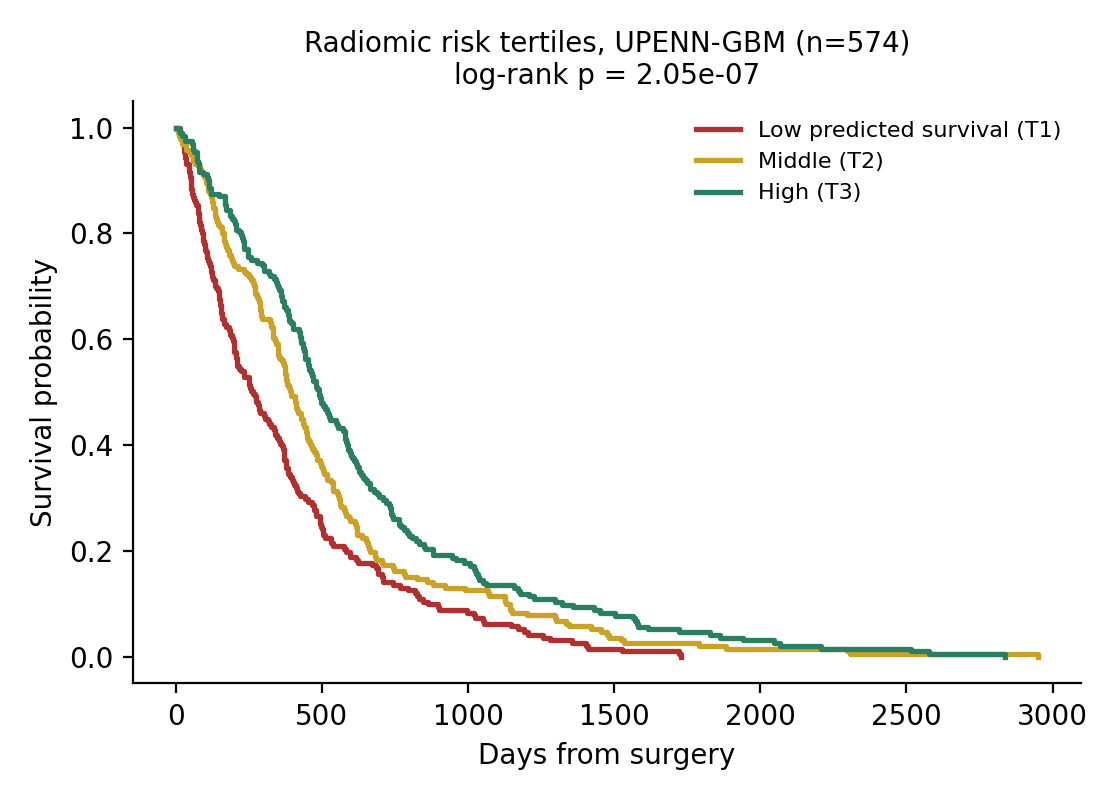
\includegraphics[width=0.63\textwidth]{fig1_km_radiomic_tertiles.png}\\[2pt]
{\footnotesize Radiomic risk tertiles, log-rank $p = 2.0\times10^{-7}$.}
\end{center}

\begin{center}
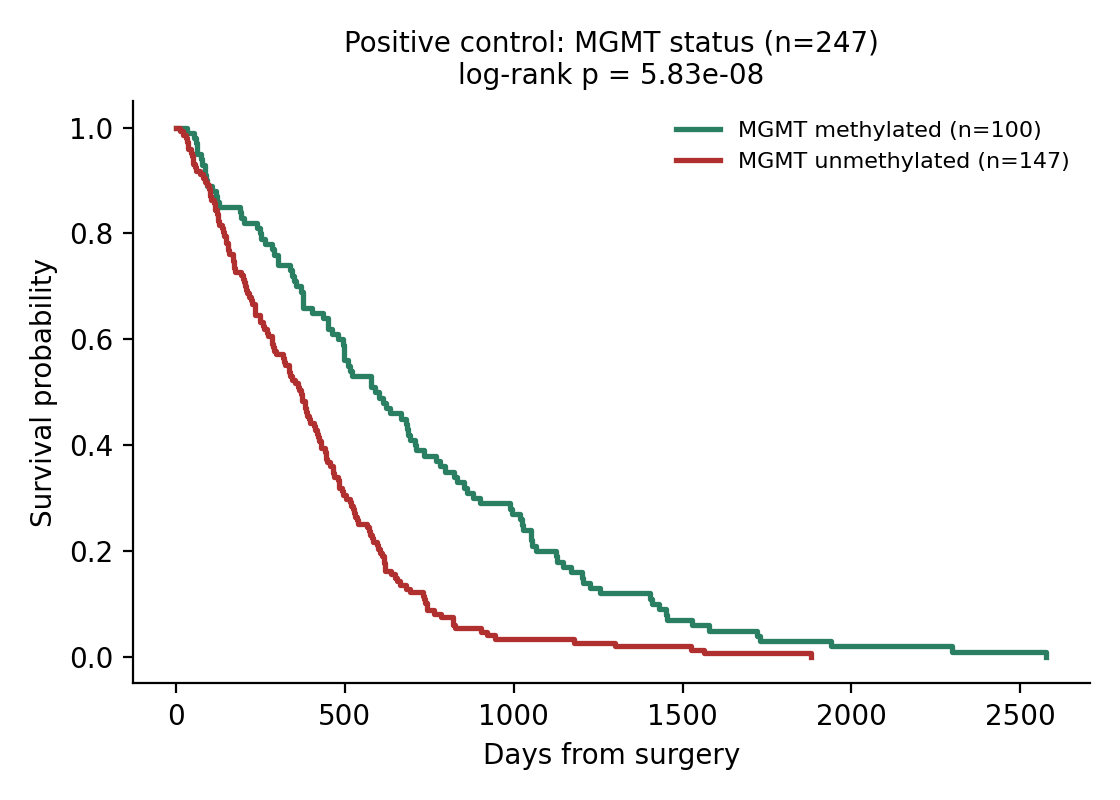
\includegraphics[width=0.63\textwidth]{fig2_km_mgmt_control.png}\\[2pt]
{\footnotesize Positive control. MGMT methylation recovers its established survival benefit.}
\end{center}

\section{Why this strengthens R01 rather than contradicting it}

R01 reported that MGMT status is not predictable from these features (AUROC 0.430, 95\% CI
0.360--0.500). A reasonable objection was that the pipeline might simply be broken. R02
answers that objection with evidence rather than assertion:

\begin{enumerate}[leftmargin=1.6em,nosep]
\item The same features and the same cross-validation machinery detect a survival signal at
$p = 0.005$ against a correctly centred null.
\item MGMT status \emph{is} biologically meaningful in this cohort --- it separates survival
at $p = 5.8\times10^{-8}$. So R01's null is not because MGMT is irrelevant here.
\item Two independent known associations were recovered at the expected effect direction.
\end{enumerate}

\noindent
The specific conclusion is therefore narrow and defensible: \textbf{radiomic appearance
tracks prognosis but does not track MGMT methylation}. Prognostic information in glioma
imaging is not reducible to this particular molecular marker.

\section{Limitations, stated plainly}

\begin{itemize}[leftmargin=1.4em,nosep]
\item \textbf{No external validation is possible with our holdings.} The 337-patient CC0
cohort intended for external validation has no survival data at all. This result is
internally validated only, and should not be presented otherwise.
\item \textbf{Uncensored by exclusion.} Patients still alive (17) have no recorded survival
time and are therefore absent. The cohort is effectively ``time to death among those who
died'', which removes censoring but introduces mild selection.
\item \textbf{Effect size is modest.} C-index 0.602 alone is below age alone (0.622). The
defensible claim is incremental value over age, not replacement of it.
\item Automatic rather than manual segmentations were used, for sample size. Segmentation
quality was not inspected.
\end{itemize}

\section{Audit}

Five checks were run after the result. Full record in \texttt{AUDIT.md}.

\begin{center}
\begin{tabular}{@{}llp{7.4cm}@{}}
\toprule
\textbf{Check} & \textbf{Verdict} & \textbf{Finding} \\
\midrule
Is it just age? & \textbf{No} & Spearman(prediction, age) $=-0.125$; radiomics adds beyond age at $p=1.6\times10^{-9}$ \\
Convergence warnings & \textbf{Immaterial} & C-index identical (0.5978) at 5{,}000 / 50{,}000 / 200{,}000 iterations \\
Leakage & \textbf{None} & Permutation null centred 0.4998 \\
Positive controls & \textbf{Both recovered} & Age and MGMT, correct directions, gate G6 \\
Gates & \textbf{7 / 7 PASS} & Including complete-case rule identical to R01 \\
\bottomrule
\end{tabular}
\end{center}

\section{How to verify}

\texttt{evidence/oof\_survival.csv} contains observed survival days and the predicted
log-survival for all 574 patients, so the C-index is recomputable directly:

\begin{verbatim}
python3 -c "
import numpy as np; from lifelines.utils import concordance_index
d=np.loadtxt('evidence/oof_survival.csv',delimiter=',',skiprows=1)
print(concordance_index(d[:,0], d[:,2]))"   # -> 0.602
\end{verbatim}

\noindent
Also included: \texttt{config.yaml} (hash \texttt{f683cfed\ldots}, written before outcomes
were read), \texttt{gates.json}, \texttt{results.json}, \texttt{audit\_permutation.json}
(all 200 null values), \texttt{cohort.json}, \texttt{inputs.json},
\texttt{MANIFEST.sha256}, \texttt{env.txt}, and \texttt{m2\_survival.py}.

\section{Recommendation}

This is the endpoint the glioma arm should be built on. It has ground truth in an imaged
cohort, it replicates known biology as a control, and it yields a modest but genuine and
age-independent signal.

Two things would materially strengthen it, both requests rather than computations:
survival data for an independent imaged cohort (none of our holdings has it), and the
UT~Southwestern images, whose 625 patients span grades 2--4 and would allow the grade
question the current cohorts cannot answer.

\vfill
\noindent{\color{qgrey}\rule{\textwidth}{0.4pt}}\\
{\footnotesize\color{qgrey}Run directory
\texttt{runs/20260806T225005Z-R02surv-3f8bece}. Data: UPENN-GBM, TCIA, CC BY 4.0
(Bakas et al., DOI 10.7937/TCIA.709X-DN49). No patient-level identifiers are reproduced.}
\end{document}
